\section{Widening link widths}
With a link width of 16 bits, the \confignoc{} can transfer 16 bits in a single cycle over a link.
Widening the links increases the amount of data that can be transferred in a single cycle.
Physically, this means that the number of wires for each link increases.
Furthermore, the routers need to be enlarged to support the change in link width.
This includes an expansion in buffer size and size of the crossbar switch. % TODO add ref
While these changes increase silicon area and power consumption, the overall impact on the system remains minimal.

\Cref{tab:latency_bandwidth_phit_width_packet_format,fig:latency_bandwidth_phit_width_packet_format} show for three different phit widths the time it takes to fill the \graicore{} and the associated effective bandwidth for the current and the improved packet format.
For the new packet format, we assume that there is minimal overhead.

\begin{table}[hbtp]
\centering
\begin{adjustbox}{width=\linewidth}
\begin{tabular}{@{}lllll@{}}
\toprule
                    & \multicolumn{2}{l}{\textbf{Latency (ms)}} & \multicolumn{2}{l}{\textbf{Effective bandwidth (GiB/s)}} \\ \cmidrule(lr){2-3} \cmidrule(lr){4-5}
\textit{Phit width} & \textit{Current packet format}    & \textit{New packet format}   & \textit{Current packet format}    & \textit{New packet format}   \\ \midrule
16                  & 47.19                    & 23.59               & 0.75                     & 1.49                \\
32                  & 23.59                    & 11.80               & 1.49                     & 2.98                \\
64                  & 11.80                    & 5.90                & 2.98                     & 5.96                \\ \bottomrule
\end{tabular}
\end{adjustbox}
\caption{Latency and effective bandwidth for different phit widths and both packet formats.}
\label{tab:latency_bandwidth_phit_width_packet_format}
\end{table}

\begin{figure}[htbp]
    \centering
    \begin{subfigure}[b]{0.48\textwidth}
        \begin{adjustbox}{width=\linewidth}
            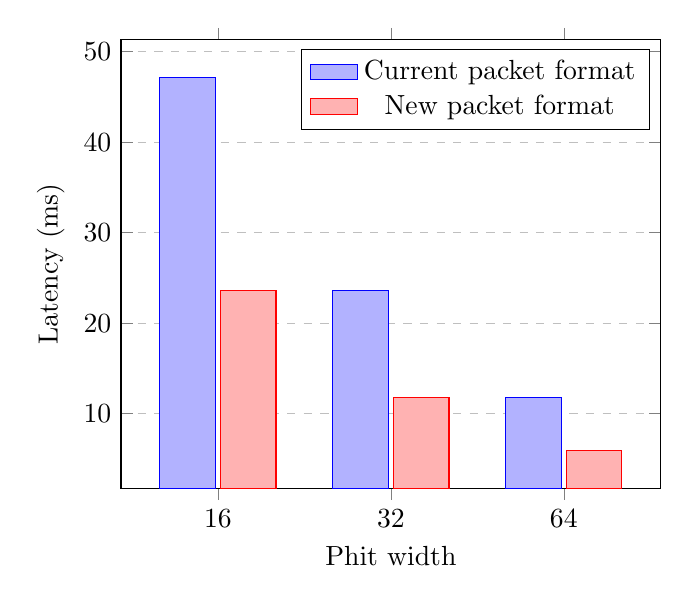
\begin{tikzpicture}
\begin{axis}[
    ylabel=Latency (ms),
    xlabel=Phit width,
    ymajorgrids=true,
    grid style=dashed,
    symbolic x coords={16, 32, 64},
    xtick={16, 32, 64},
    ybar,
    enlarge x limits={abs=35pt},
    bar width=20pt
]

\addplot+[
area legend,
] 
	coordinates {
            (16,47.19)
            (32,23.59)
    	  (64,11.80)
        };
\addplot+[
area legend,
] 
	coordinates {
            (16,23.59)
            (32,11.80)
    	  (64,5.90)
        };
\legend{Current packet format, New packet format}
\end{axis}
\end{tikzpicture}
        \end{adjustbox}
        \caption{Latency}
    \end{subfigure}
    \hfill
    \begin{subfigure}[b]{0.48\textwidth}
        \begin{adjustbox}{width=\linewidth}
            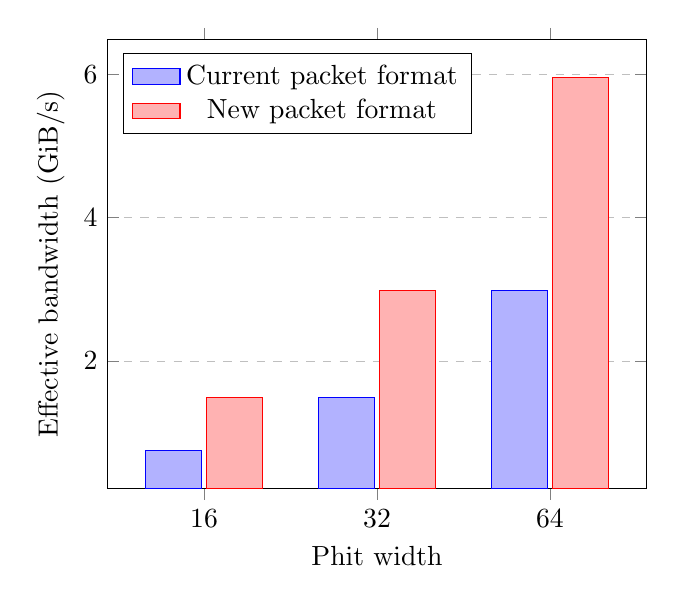
\begin{tikzpicture}
\begin{axis}[
    ylabel=Effective bandwidth (GiB/s),
    xlabel=Phit width,
    ymajorgrids=true,
    grid style=dashed,
    symbolic x coords={16, 32, 64},
    xtick={16, 32, 64},
    ybar,
    enlarge x limits={abs=35pt},
    bar width=20pt,
    legend pos=north west,
]

\addplot+[
area legend,
] 
coordinates {
        (16,0.75)
        (32,1.49)
        (64,2.98)
};
\addplot+[
area legend,
] 
coordinates {
    (16,1.49)
    (32,2.98)
    (64,5.96)
};
\legend{Current packet format, New packet format}
\end{axis}
\end{tikzpicture}
        \end{adjustbox}
        \caption{Effective bandwidth}
    \end{subfigure}
    \caption[]{For both the old and newly proposed packet formats, the latency is shown for various phit widths}
    \label{fig:latency_bandwidth_phit_width_packet_format}
\end{figure}
